\section {Оценка выходных погрешностей}

Для оценки точности автономной работы БИНС на базе кластерного блока чувствительных элементов были использованы уравнения ошибок автономной работы ИНС. Данные уравнения учитывают медленно изменяющуюся составляющую ошибки, не зависящую от горизонтального ускорения объекта. Нестационарные погрешности, зависящие от ускорения и обусловленные погрешностью масштабных коэффициентов акселерометров, представляют собой высокочастотную ошибку, модулирующую медленно изменяющуюся шулеровскую, не учитываются в данной модели. 


Для связи выходных параметров ИНС (крен, тангаж, курс, широта, долгота) использованы следующие зависимости:  


\begin{equation}
	\label{eq:phi_x}
	\begin{gathered}
		\varPhi_x(t) = \varPhi_x(0) \cos \nu t - 
		U \cos \phi \frac {\sin \nu t} {\nu} \varPhi_z(0) - 
		\frac{\sin \nu t}{ \nu R} \delta V_y(0) +
		\frac{\sin \nu t}{\nu} \xi_x -\\ 
		U \cos \varPhi \frac{1-\cos \nu t}{\nu^2}\xi_z - 
		\frac{1-\cos \nu t}{\nu^2R} B_y(0)
	\end{gathered}
\end{equation}


\begin{equation}
	\label{eq:phi_y}
		\begin{gathered}
		\varPhi_y(t) = \varPhi_y(0) \cos \nu t + 
		\frac {\sin \nu t} {\nu R} \delta V_x(0) +
		\frac{\sin \nu t}{\nu} \xi_y +\\  
		\frac{1 - \cos \nu t}{ \nu^2 R} B_y(0)
	\end{gathered}
\end{equation}


\begin{equation}
	\label{eq:phi_z}
	\begin{gathered}
		\varPhi_z(t) = \varPhi_x(0) U \cos \phi t + 
		\varPhi_y(0) \tg \phi + \frac{ \tg \phi \sin \nu t }{ \nu R } \delta V_x(0) - \\
		(t - \frac{\sin \nu t}{\nu}) \tg \phi \xi_y + \tg \phi \frac{ 1-\cos \nu t }{ \nu^2 R } B_x(0) + \\
		\varPhi_z(0) + \xi_z t
	\end{gathered}
\end{equation}


\begin{equation}
	\label{eq:V_e}
	\begin{gathered}
		\delta V_e(t) = - \varPhi_y(0) R \sin \nu t + \delta V_x(0) \cos \nu t - \xi_y R (1 - \cos \nu t) + \\
		\frac{\sin \ nu t}{ \nu } B_x(0)
	\end{gathered}
\end{equation}


\begin{equation}
	\label{eq:V_n}
	\begin{gathered}
		\delta V_n(t) = - \varPhi_x(0) R \sin \nu t + \delta V_y(0) \cos \nu t + \xi_x R (1 - \cos \nu t) + \\
		\frac{\sin \ nu t}{ \nu } B_y(0)
	\end{gathered}
\end{equation}

\begin{equation}
	\label{eq:lambda}
	\begin{gathered}
		\lambda (t) = \int \frac{\delta V_e(t)}{R \cos \phi} dt
	\end{gathered}
\end{equation}

\begin{equation}
	\label{eq:phi}
	\begin{gathered}
		\phi (t) = \int \frac{\delta V_n(t)}{R \cos \phi} dt
	\end{gathered}
\end{equation}


\vspace{0.5cm}
где { \large $ \nu = \sqrt{ \frac{g}{R} } $ } - шулеровская частота колебания;


\vspace{0.5cm}
{\large $ B_x(0), B_y(0) $} - смещения нулей акселерометра;


\vspace{0.5cm}
{\large $ \xi_x, \xi_y, \xi_z $} - дрейф гироскопа;


\vspace{0.5cm}
Для оценки остаточной случайной составляющей погрешности акселерометра и гироскопа, с целью использования
данных значений в уравнениях  ~(\ref{eq:phi_x}) --- ~(\ref{eq:phi}) проведена запись показаний чувствиетльных элементов на протяжении 2-ух часов. По результатам измерений построены графики девиации Аллана. 

\newpage

\begin{figure}[h!]
	\centering
	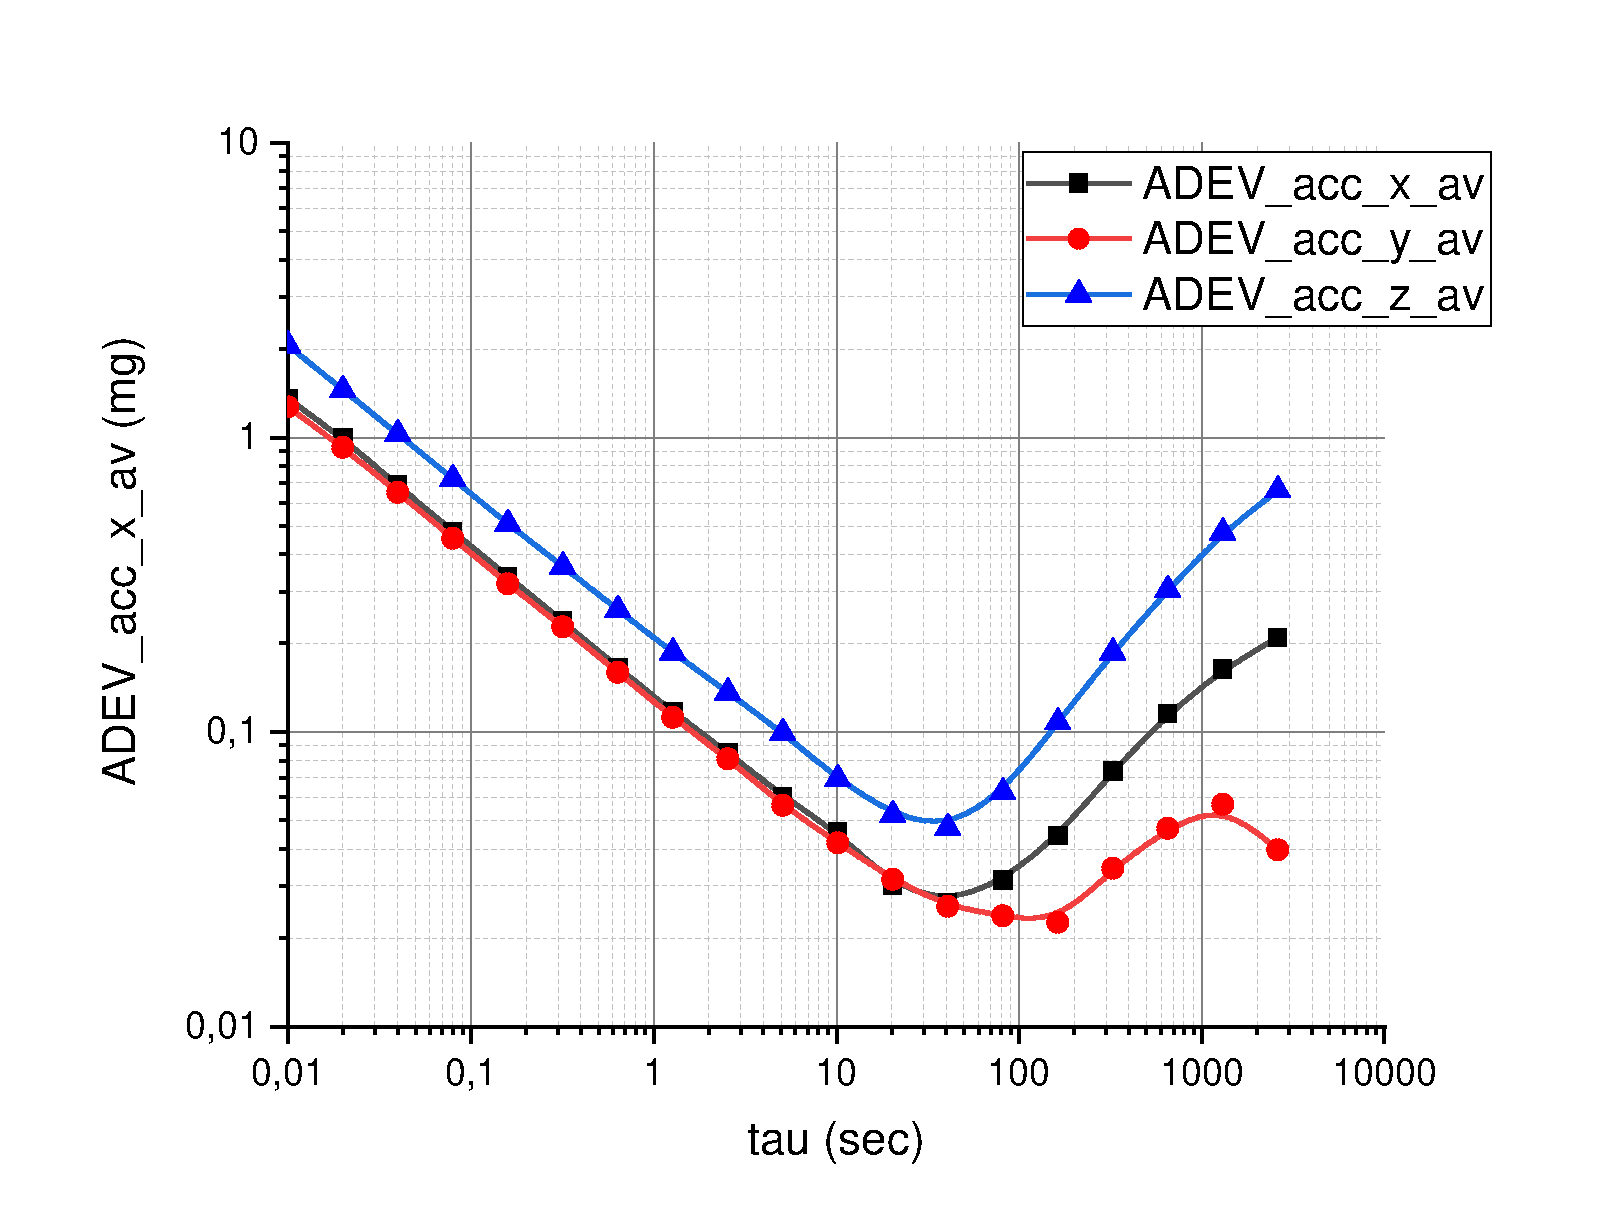
\includegraphics[width=0.9\linewidth]{acc_av_adev.pdf}
	\caption{График девиации Аллана}
	\label{fig:accAdev}
\end{figure}


Полученный график Рис.\ref{fig:accAdev} девиации Аллана позволяет оценить остаточную случайную погрешность, которая будет присутствовать в выходных данных показаний акселерометров в составе кластерного инерциального измерительного блока. Исходя из уравнений ~(\ref{eq:phi_x}) -- ~(\ref{eq:phi}) остаточная погрешность акселерометра не вносит существенный вклад в ошибку определения выходных координат. Данная ошибка будет влиять исключительно на расчет пространственной ориентации.  


Ниже представлены графики нарастания ошибки определения угла тангажа и крена в течение 5 секунд автономной работы кластерной инерциальной навигационной системы. 

\newpage

\begin{figure}[h!]
	\centering
	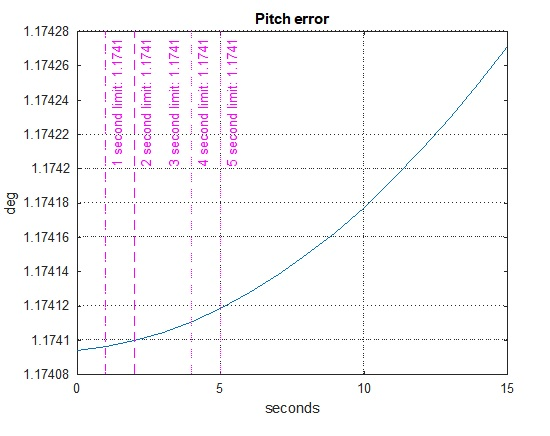
\includegraphics[width=0.7\linewidth]{pitch.png}
	\caption{Нарастание ошибки в определении тангажа}
	\label{fig:pitch}
	
	\vspace*{\floatsep}
	
	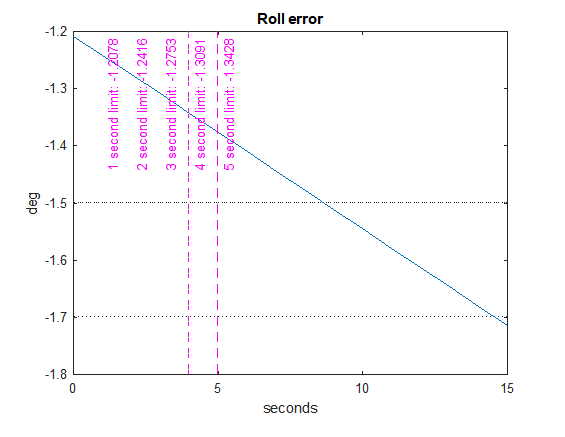
\includegraphics[width=0.7\linewidth]{roll.png}
	\caption{Нарастание ошибки в определении крена}
	\label{fig:roll}
	
\end{figure}

\newpage
Дрейф гироскопов является основной составляющей ошибки определения координат в процессе автономной работы ИНС. Именно поэтому основной задачей исследования точности чувствительных элементов был анализ остаточных погрешностей гироскопов. Из графика (Рис.\ref{fig:mpr}) видно, что значение дрейфа на интервале осреднения 0.01 с. не превышает 0.03375 \SI[per-mode=symbol]{}{\degree\per\second}


\begin{figure}[h!]
	\centering
	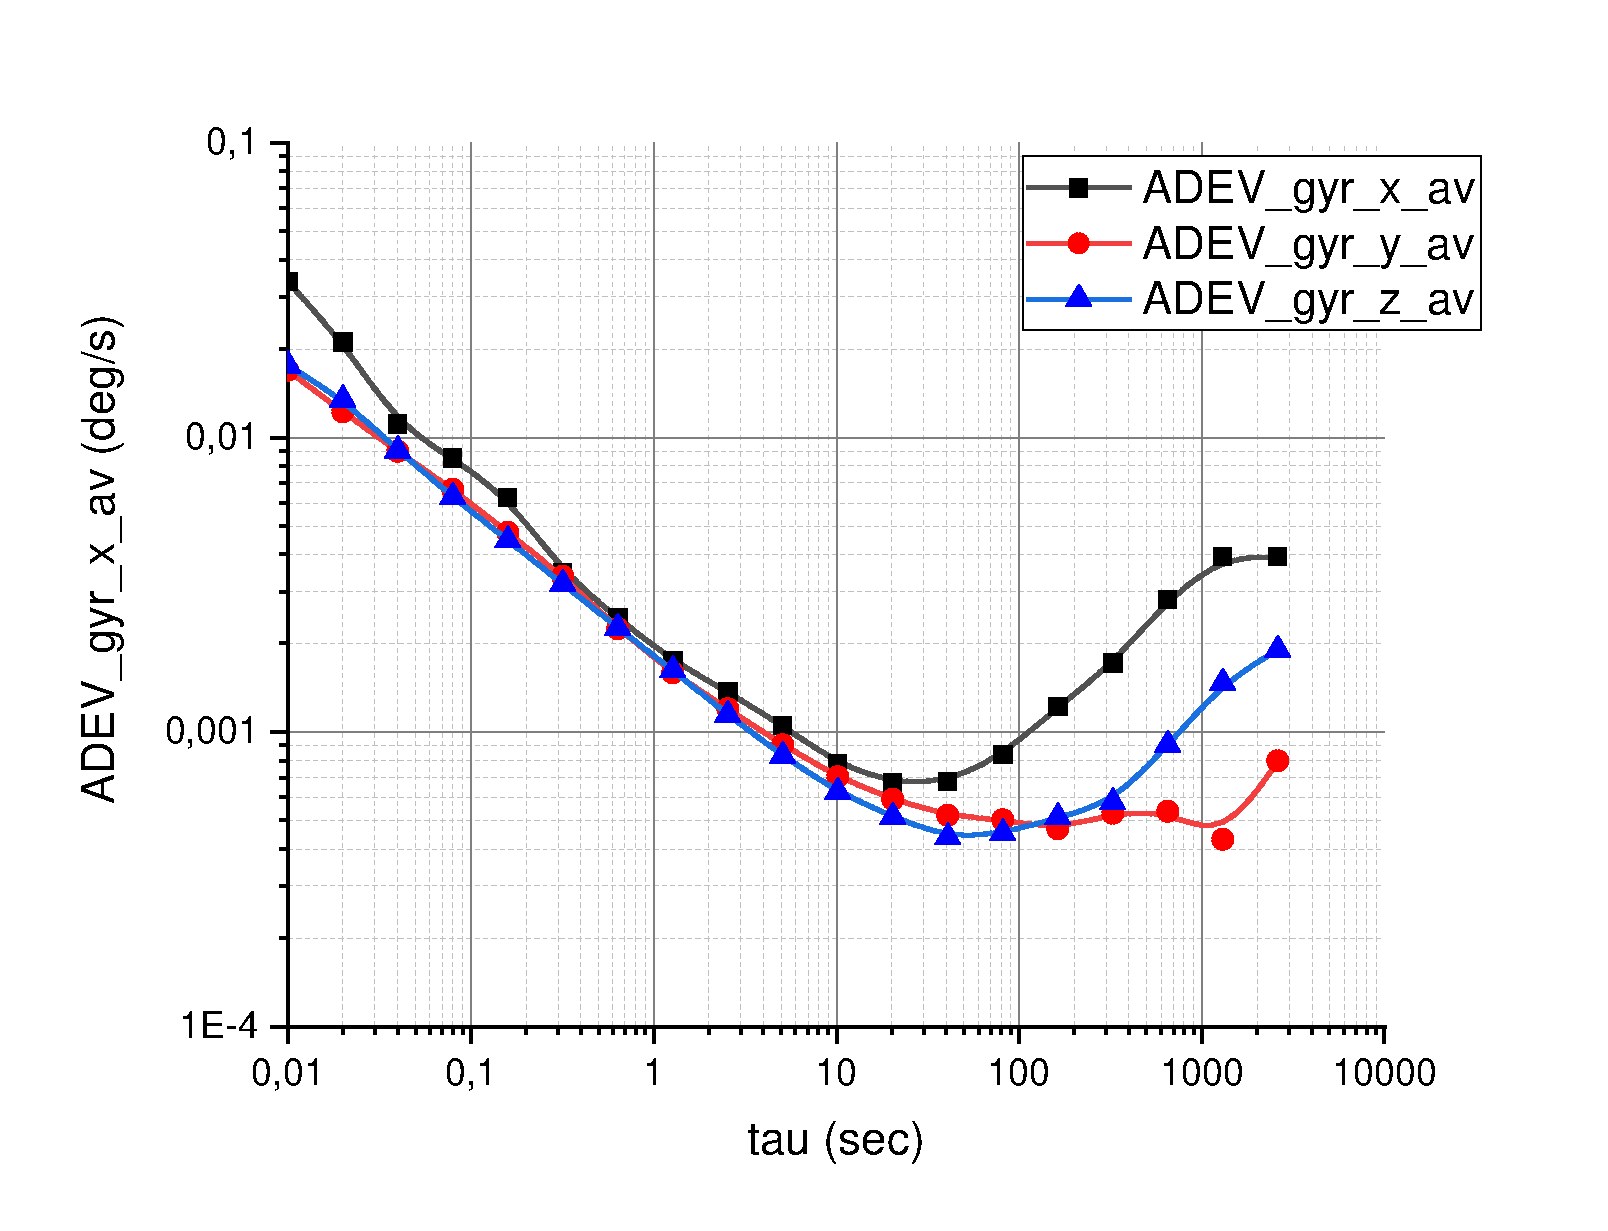
\includegraphics[width=0.9\linewidth]{gyr_av_adev.pdf}
	\caption{График девиации Аллана}
	\label{fig:mpr}
\end{figure}

\newpage

\begin{figure}[h!]
	
	\centering
	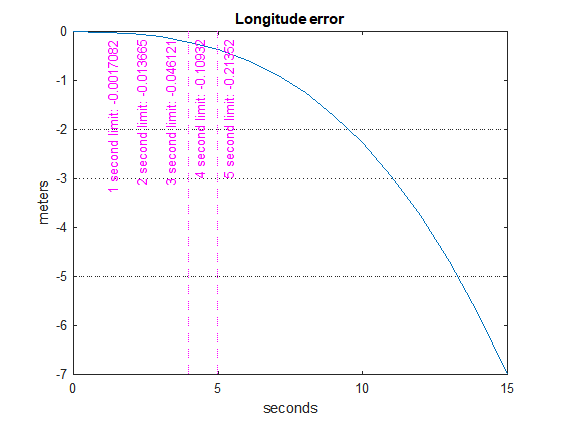
\includegraphics[width=0.8\linewidth]{longitudeError.png}
	\caption{График нарастания ошибки в определении долготы места}
	\label{fig:long_error}

	\vspace*{\floatsep}
	
	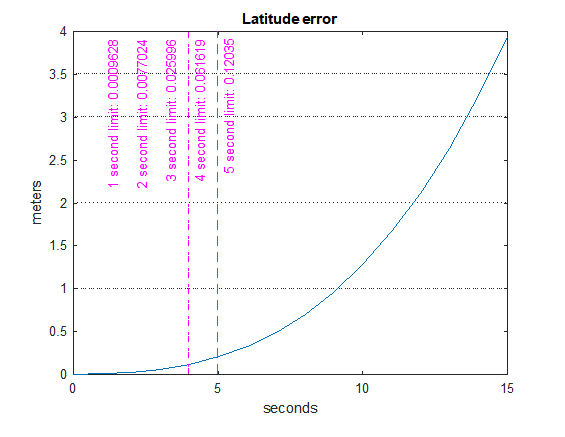
\includegraphics[width=0.8\linewidth]{latitudeError.png}
	\caption{График нарастания ошибки в определении широты места}
	\label{fig:lat_error}
\end{figure}
\newpage
